% Rule sheet for primes game
% Game design: Grant Sinclair
% Graphic design: Harald Bögeholz

\documentclass{article}

\usepackage{fontspec}
\usepackage{graphicx}
\usepackage{adjustbox}

\setmainfont{HelveticaNeue}

\newcommand{\card}[1]{\adjustbox{valign=m}{\includegraphics[page=#1, width=2cm]{primecards-screen.pdf}}}
\newcommand{\largecard}[1]{\adjustbox{valign=m}{\includegraphics[page=#1, width=37mm]{primecards-screen.pdf}}}
\newcommand{\square}[1]{\adjustbox{valign=m}{
\includegraphics[page=#1, width=2cm]{boardsquares.pdf}}}

\setlength{\parindent}{0pt}

\begin{document}


\section*{Setup}

Each player starts with a single meeple on the starting square. Shuffle the deck, deal two cards to each player and place the deck black side up. Players should hold their cards so only they can see the symbols on the white sides of their cards, but the numbers of the black sides are visible to their opponents.

\section*{Gameplay}

Players take turns in a clockwise direction. On their turn, a player may \textbf{trip} a square that contains their opponent’s meeple by playing any number of cards white side up so that the symbols exactly match the symbols on the square with the opponent’s meeple.

Each opponent’s meeple on the tripped square is moved back by the sum of the numbers on the cards played, and the player \textbf{draws a card for each meeple tripped}. A meeple cannot be tripped below zero and will stop at the starting square rather than be tripped further back. The player may continue tripping opponents as long as they can. After that, the player may play a single card black side up, or not, and move their meeple forward by the sum of the numbers on all the cards they have played this turn. Meeples cannot be moved beyond 100; if a meeple is too close to 100 and the number is too large, the meeple has to stay in place. 

\textbf{At the end of their turn, the player draws two cards.} All played cards are now discarded. Discarded cards are not reused during the game. When the draw pile runs out, players just stop drawing, forcing them to pass eventually. 
 
\section*{End of the game}

The game ends when a player gets to 100, when all players pass on consecutive turns, or after a specified time limit. The winner is the player whose meeple is furthest ahead.

\section*{Example turn}

Let's say on a player's turn there is one opponent meeple on square \square{12} and one opponent meeple on square~\square{5}.

The player trips by playing \card{91} \card{69} for a total of 7, taking one opponent meeple from \square{12} back to \square{5}, and draws a card for tripping.

The player now trips again by playing \card{125}, sending \textbf{two} opponent meeples back from \square{5} to the starting square, and draws two cards for tripping two meeples.

Finally, the player plays~\card{170} and moves their meeple forward 21 squares, the sum of all the numbers played. They draw two cards at the end of their turn and discard all the cards from play.

\section*{Optional rule: Mercy}

The meeple in the last position cannot be tripped.

\section*{Advanced Rules for 2--3 players}

Rules are the same as above unless noted.

For two players, each player has three meeples of the same colour. For three players, each player has two meeples of the same colour.

The deck is cut after shuffling. The Mercy rule does not apply. 

The winner is the player whose \textbf{last meeple is furthest ahead} when the game ends. 

If that is equal, the tie can be broken by the second-last meeple. If that is also equal in a two-player game, the tie can be broken by the first meeple. If all meeples are on the same squares, those players draw the game.

Players cannot move a meeple to 100 unless doing so wins them the game.


\section*{Team play for 4 players (2 teams of 2)}

Rules are the same as the Advanced Rules unless noted.

Players sit opposite their partner. 

Partners are not allowed to communicate with each other.

Each pair of players has three meeples of the same colour.

\section*{About the cards}

The deck has 108 cards, 12 for each number from 1 to~9. For each number, the back (black side) of the card shows which 12 symbols (or combinations of symbols) are on the white side of cards with that number.

\begin{centering}
\begin{tabular}{ccc}
\vspace*{5pt}\\
\largecard{2} & \largecard{26} & \largecard{50} \vspace*{10pt}\\
\largecard{74} & \largecard{98} & \largecard{122} \vspace*{10pt}\\
\largecard{146} & \largecard{170} & \largecard{194} \vspace*{10pt}\\
\end{tabular}
\end{centering}

\end{document}
